\subsection{Supported magnitude-frequency distributions}
\label{sec:mfd}
The magnitude-frequency distributions currently supported by the 
\gls{acr:oqe} are the following: 
\begin{description}
    \item[A discrete incremental magnitude-frequency distribution] \hfill \\
    It's the simplest distribution offered. It's defined by a 
    minimum value of magnitude (representing the mid point of the first
    bin) and the bin width. The distribution itself is simply a 
    sequence of floats describing the annual number of events for 
    different bins (centered on increasing values of magnitude). 
    Below we show an example of the xml used to describe an incremental 
    \glspl{acr:mfd} for a seismic source input of a \gls{acr:ssim}.
\begin{Verbatim}[frame=single, commandchars=\\\{\}, fontsize=\footnotesize]
<incrementalMFD minMag="5.05" binWidth="0.1">
    <occurRates>0.15 0.08 0.05 0.03 0.015</occurRates>
</incrementalMFD>
\end{Verbatim}
    This is the magnitude-frequency distribution obtained with the above
    settings:
% ..............................................................................
% . . . . . . . . . . . . . . . . . . . . . . . . . . . . . . . . . . . > Figure
\begin{figure}[!ht]
\centering
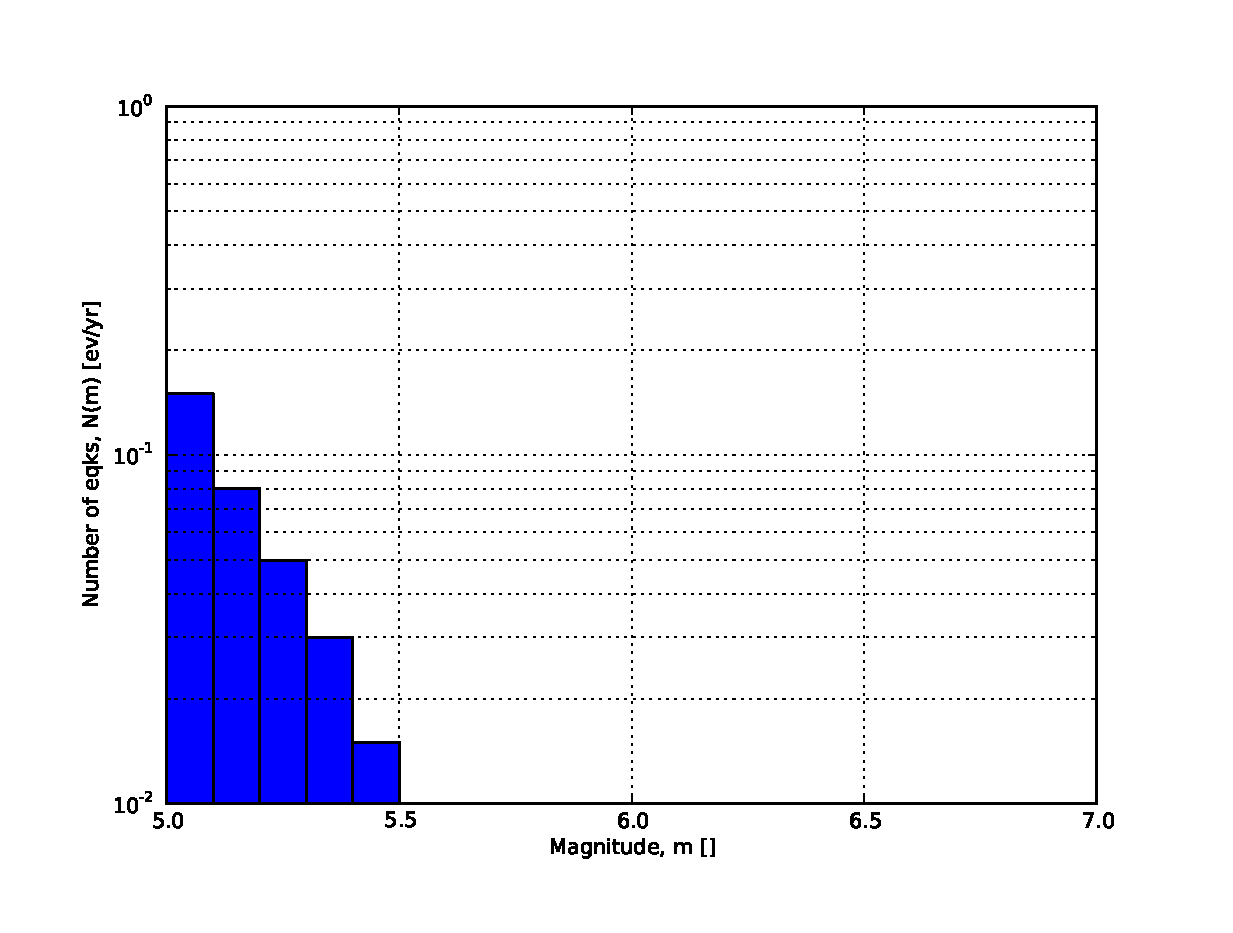
\includegraphics[width=12cm]{./figures/hazard/ed_mfd.eps}
\caption{Incremental magnitude-frequency distribution.}
\label{fig:evenly_discretized_mfd}
\end{figure}
% . . . . . . . . . . . . . . . . . . . . . . . . . . . . . . . . . . . < Figure
% ..............................................................................
%
\item[A double truncated Gutenberg-Richter distribution] \hfill \\
    This distribution is de\-scribed by means of a minimum \texttt{minMag}
    and maximum magnitude \texttt{maxMag} and by the $a$ and $b$ values 
    of the Gutenberg-Richter relationship. The synthax of the xml is 
    rather compact as shown below
\begin{Verbatim}[frame=single, commandchars=\\\{\}, fontsize=\footnotesize]
<truncGutenbergRichterMFD aValue="5.0" bValue="1.0" minMag="5.0" 
        maxMag="6.0"/>
\end{Verbatim}
    This is the magnitude-frequency distribution obtained using the 
    parameters of the considered example:
% ..............................................................................
% . . . . . . . . . . . . . . . . . . . . . . . . . . . . . . . . . . . > Figure
\begin{figure}[!ht]
\centering
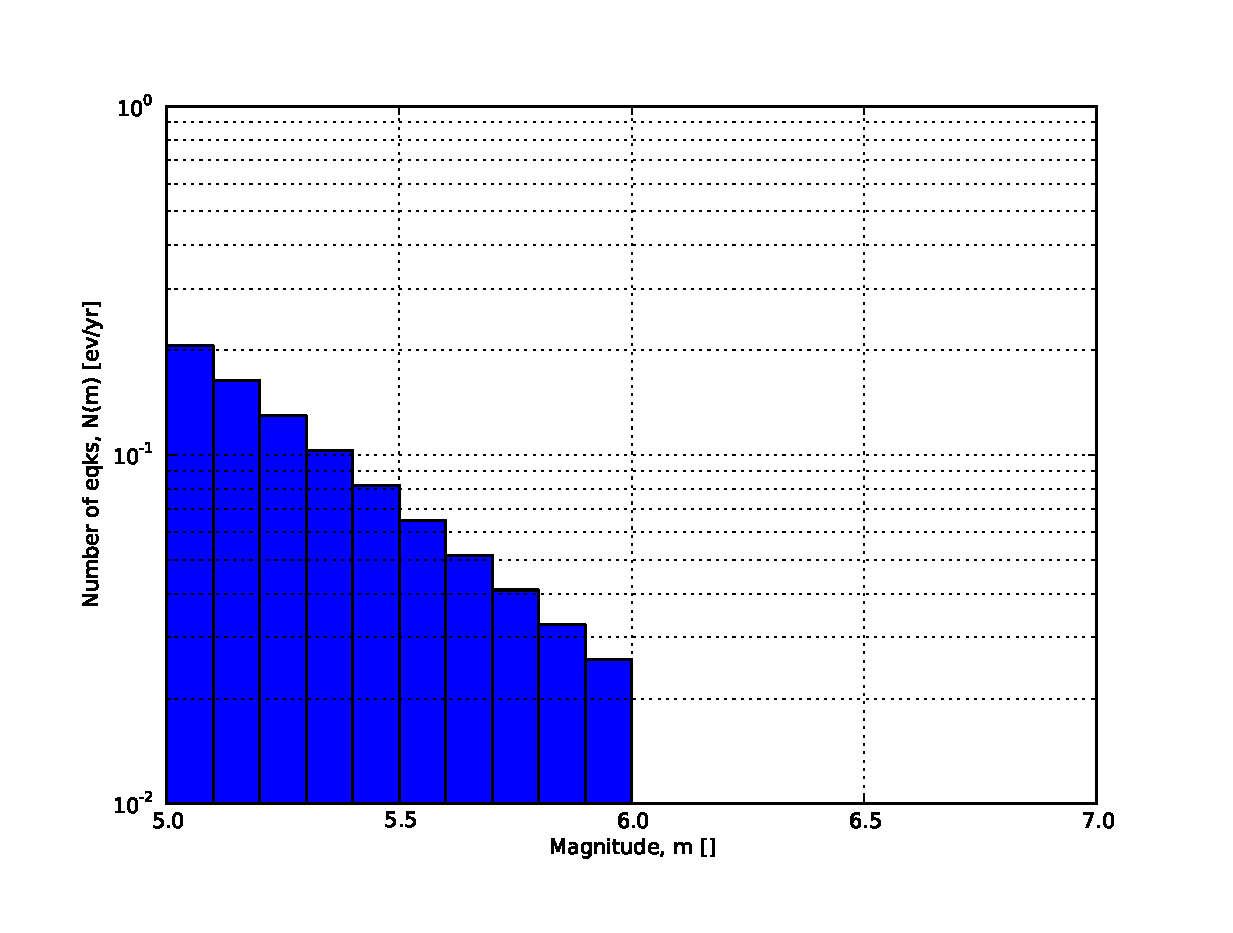
\includegraphics[width=12cm]{./figures/hazard/dt_mfd.eps}
\caption{Double truncated Gutenberg-Richter magnitude-frequency distribution.}
\label{fig:dt_gr_mfd}
\end{figure}
% . . . . . . . . . . . . . . . . . . . . . . . . . . . . . . . . . . . < Figure
% ..............................................................................
%
\item[Characteristic earthquake model (\`{a} la \cite{youngs1985})]
    The 
\begin{Verbatim}[frame=single, commandchars=\\\{\}, fontsize=\footnotesize]
    AA
\end{Verbatim}
% ..............................................................................
% . . . . . . . . . . . . . . . . . . . . . . . . . . . . . . . . . . . > Figure
\begin{figure}[!ht]
\centering
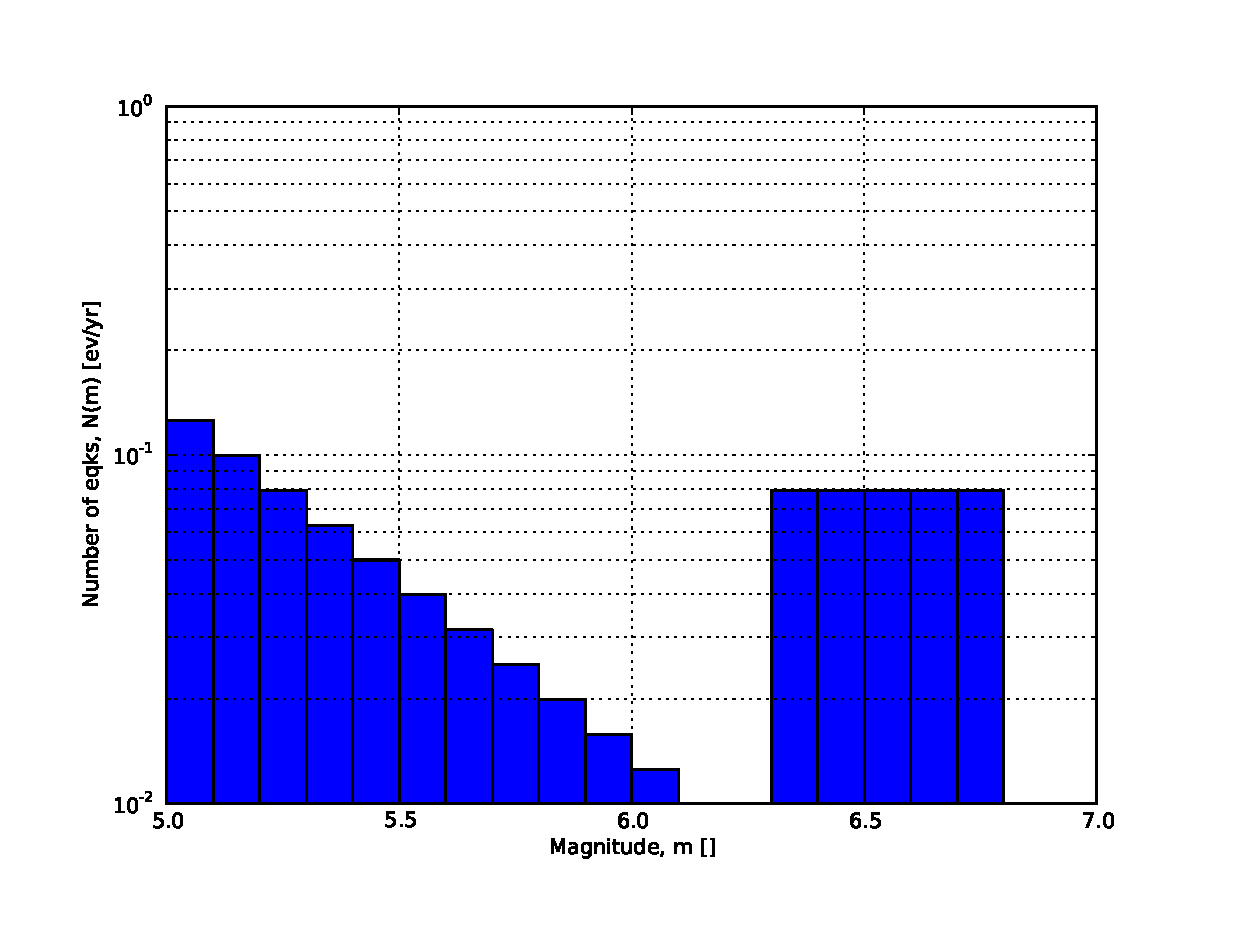
\includegraphics[width=12cm]{./figures/hazard/yc_mfd.eps}
\caption{\cite{youngs1985} magnitude-frequency distribution.}
\label{fig:yc_gr_mfd}
\end{figure}
% . . . . . . . . . . . . . . . . . . . . . . . . . . . . . . . . . . . < Figure
% ..............................................................................

\end{description}
